\begin{problem}{Швея Севера}{стандартный ввод}{стандартный вывод}{1 секунда}{256 мегабайт}

Петя уже давно занимается в робототехническом кружке. Нынче осенью он 
сконструировал швейного робота для фабрики «Сардаана». Робот должен изготавливать прямоугольные панно, сшивая их из одинаковых квадратных черных и белых лоскутков. Узор на панно образует две раскручивающиеся по часовой стрелке спирали. Он начинается 
с черного квадратика, пришитого снизу к белому, причем первый отрезок черной спирали «вырастает» влево из первого черного квадратика (см. рис.). 
\\~

\noindent\medskip\centerline{
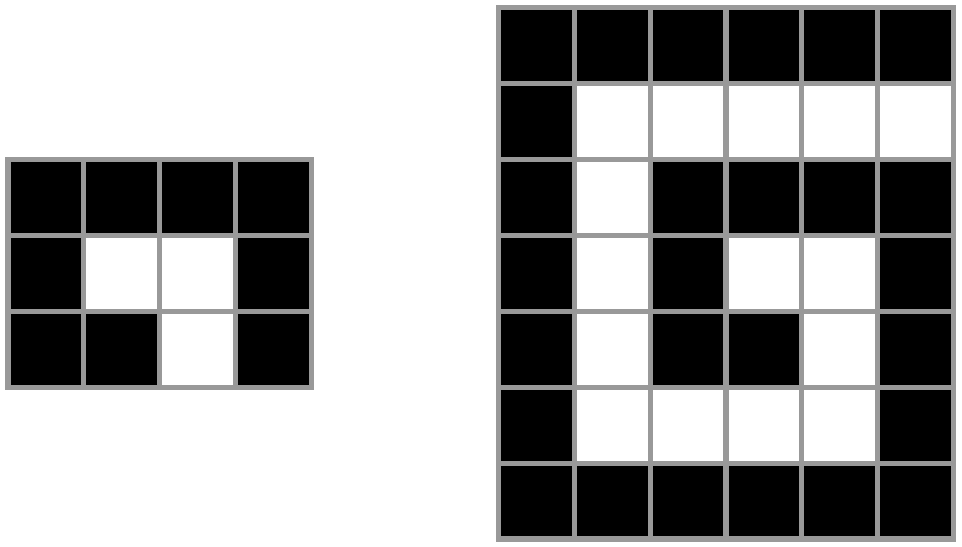
\includegraphics[bb=0 0 16.29cm 9.27cm, scale=.4]{loskut.pdf}
}
\centerline{Панно для $n = 4$ и $n = 7$}

Известно требуемое число $n$ прямолинейных отрезков черной спирали.  При этом первые $n-1$ из них полные, и их невозможно удлинить, продолжив спираль. Последний же отрезок -- укороченный исходя из того, что белый материал дороже, поэтому белая спираль делается как можно короче при данном~$n$.

Поскольку память робота невелика, надо научиться сшивать панно по частям. Помогите Пете написать программу, которая выведет карту клеток в заданной части панно.

\InputFile
Первая строка содержит одно целое число $n$ ($3 \leq n \leq 10^6$)~--- требуемое количество прямолинейных отрезков черной спирали панно.  Во второй строке записаны через пробел четыре натуральных числа $l$, $t$, $w$ и $h$ ($1 \leq w, h \leq 500$)~--- номер столбца и строки, считая с единицы, содержащего левую верхнюю клетку интересующей робота сейчас области, а также ширина и высота этой области соответственно. Гарантируется, что область находится целиком в пределах панно для данного~$n$.

\OutputFile
Выведите карту заданной области  лоскутного панно в виде $h$ строк равной длины, составленных из нулей или единиц без пробелов, по $w$ цифр в строке. Черному квадратику соответствует 1, белому~--- 0.

\Examples

\begin{example}
\exmpfile{example.01}{example.01.a}%
\exmpfile{example.02}{example.02.a}%
\end{example}

\end{problem}

